\chapter{Elektronik}

\renewcommand{\kapitelautor}{Autor: Lucas Ullrich}

\section{Blockschaltbild}
An einen PIC18F46K22 werden diverse Module angeschlossen. Darunter ein Wlan-Modul, eine Kamera, ein Ultraschallsensor sowie ein Empfänger einer Fernsteuerung und ein Flighcontroler.
\begin{figure}[H]
\begin{centering}
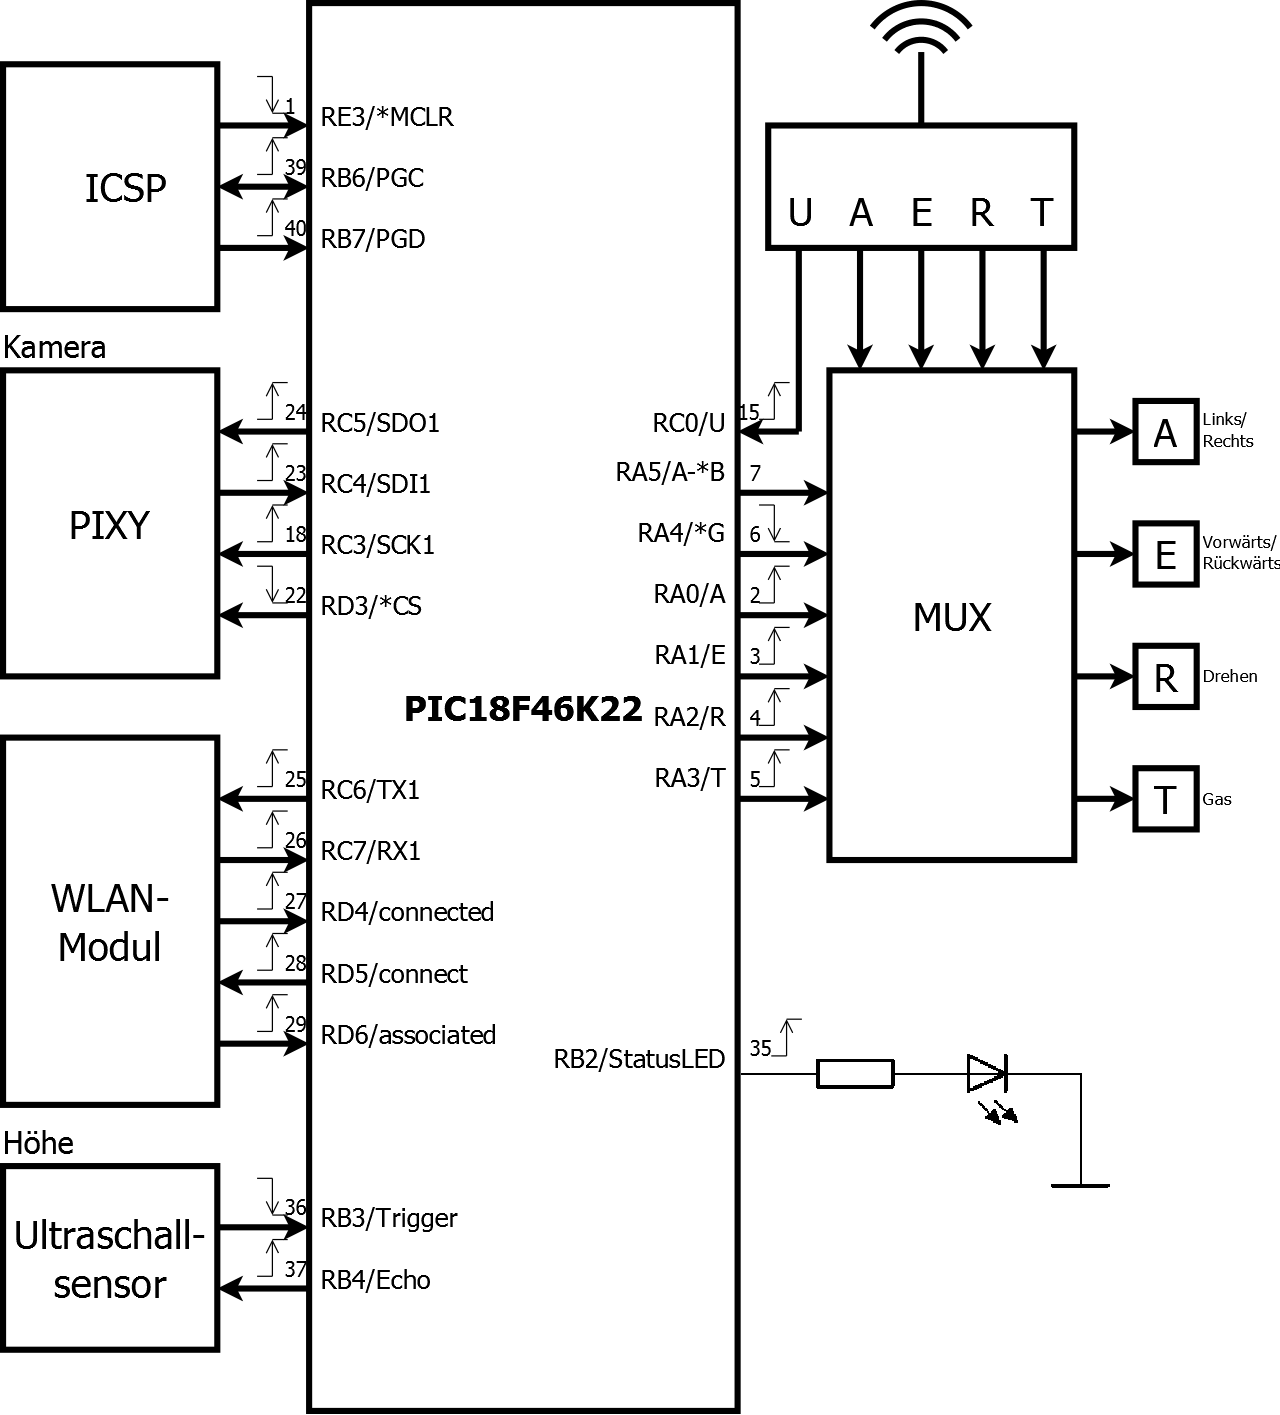
\includegraphics[width = 0.8\textwidth]{Bilder/Blockbild}
\par\end{centering}
\caption{Blockschaltbilder der Hauptplatine}
\label{Blockschaltbild}
\end{figure}

%\needspace{3cm}
\section{Sensoren}
Um einen autonomen Flug zu realisieren sind unterschiedliche Sensoren notwendig.
Durch die Sensoren muss es möglich sein die aktuelle Flugposition im Raum zu bestimmen und so den richtigen Weg zu finden.

\subsection{Kamera}
Aufgrund der Zuverlässigkeit einer Kamera im Vergleich zu Systemen die auf Distanzmessungen basieren wurde für die generelle Wegfindung das Kameramodul PIXY cmucam5 gewählt. Dieses gibt die notwendigen Informationen bereits fertig ausgewertet aus. Es wird ein Objektcode, dessen Position auf dem Bild sowie die Objektgröße wiedergegeben.
Anhand dieser Informationen und einer vorher zugesendeten Route kann der Weg zum Ziel bestimmt werden.

\begin{figure}[tbh]
\begin{centering}
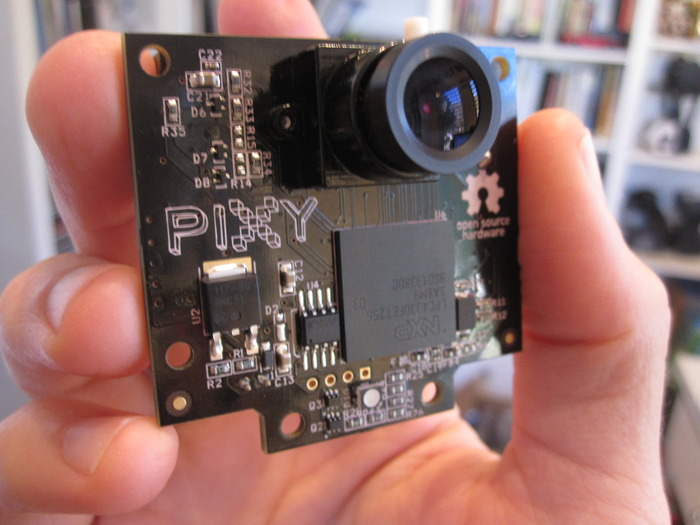
\includegraphics[width = 0.5\textwidth]{Bilder/PIXY}
\par\end{centering}
\caption{Kamera PIXY cmucam5}
\label{PIXY}
\end{figure}

\subsection{Ultraschallsensor}
Da das Bestimmen der Flughöhe durch die Kamera zwar möglich ist, sich aber sehr aufwändig gestaltet, es müssen diverse Objektparameter bekannt sein und es besteht ein hoher Rechenaufwand, wird für die Messung der Flughöhe ein Ultraschallsensor verwendet. Dieser bietet die Möglichkeit die Flughöhe auf eine Distanz von bis zu 3 m zu bestimmen.

\begin{figure}[tbh]
  \begin{centering}
    \subfigure[Beschaltung]{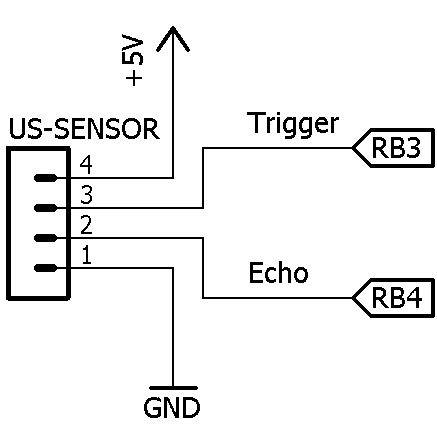
\includegraphics[width = 0.3\textwidth]{Bilder/US-Sensor}}
    \subfigure[Messsignale]{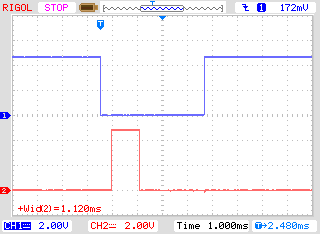
\includegraphics[width = 0.3\textwidth]{Bilder/Ultraschallmessung}}
  \par\end{centering}
  \caption{Messung mit einem Ultraschallsensor}
  \label{Ultraschallmessung}
\end{figure}

Die Messung mit dem Ultraschallsensor erfolgt nach einem Triggerimpuls (blau dargestellt)welcher low-active ist und mindestens 6 µs andauert. Nach einer Verzögerung von einigen 100 µs sendet der Sensor einen "Ultraschallburst" aus.
\\Siehe \url{http://mikrocontroller.net/}\footnote{\url{http://www.mikrocontroller.net/attachment/218122/HC-SR04_ultraschallmodul_beschreibung_3.pdf} 11/01/2016 14:16}

\needspace{2cm}
Der bei dieser Messung zurückgegebene Impuls (rot dargestellt), auch "Echo" bezeichnet, liefert die Zeit zurück die der ausgesendete Ultraschallburst benötigt hat um wieder bis zu dem Empfänger zurückzukehren. Folglich wird mit dem Ultraschallsensor die dopplete Strecke gemessen.
Mit einer Schallgeschwindigkeit von $343$ $\frac{m}{s}$ ergibt sich zur Berechnung des gemessenen Abstands folgende Formel:
\[
s = \frac{v \cdot t}{2} = \frac{343 \cdot time\_high}{2}
\]
